\documentclass[first=dgreen,second=purple,logo=redque]{aaltoslides}
%\documentclass{aaltoslides} % DEFAULT
%\documentclass[first=purple,second=lgreen,logo=redque,normaltitle,nofoot]{aaltoslides} % SOME OPTION EXAMPLES

\usepackage[latin9]{inputenc}
\usepackage[T1]{fontenc}
\usepackage{graphicx}
\usepackage{amssymb,amsmath}
\usepackage{url}
\usepackage{lastpage}
\usepackage{subfigure}
\usepackage{algpseudocode}
\usepackage{xcolor}

\definecolor{dgreen}{rgb}{0.,0.6,0.}

\newcommand\overmat[2]{%
  \makebox[0pt][l]{$\smash{\color{white}\overbrace{\phantom{%
    \begin{matrix}#2\end{matrix}}}^{\text{\color{black}#1}}}$}#2}
\newcommand\bovermat[2]{%
  \makebox[0pt][l]{$\smash{\overbrace{\phantom{%
    \begin{matrix}#2\end{matrix}}}^{\text{#1}}}$}#2}
\newcommand\partialphantom{\vphantom{\frac{\partial e_{P,M}}{\partial w_{1,1}}}}

\title{Simple and Deterministic Matrix Sketching\footnote{Authored by Edo Liberty and and won the \textit{KDD-2013 best paper} award\cite{Liberty13}.}}

\author[H. Georgiev and H. Shen]{Hristo Georgiev and Huibin Shen}
\institute[ICS]{Department of Information and Computer Science\\
Aalto University, School of Science}

\aaltofootertext{H. Georgiev and H. Shen}{T-61.6020}{\arabic{page}/\pageref{LastPage}\ }

%\date{}
\newcommand{\vectornorm}[1]{\left\|#1\right\|}
\newcommand{\IndState}{\State\hspace{\algorithmicindent}}

\everymath\expandafter{\the\everymath \color{blue}}

\begin{document}

%%%%%%%%%%%%%%%%%%%%%%%%%%%%%%%%%%%%%%%%%%%%%%%%%%%%%%%%%%%%%%%%%%%%%%%%%%%%%%%%%%%%%%%%%%%%%

\aaltotitleframe

%%%%%%%%%%%%%%%%%%%%%%%%%%%%%%%%%%%%%%%%%%%%%%%%%%%%%%%%%%%%%%%%%
% Background section
%%%%%%%%%%%%%%%%%%%%%%%%%%%%%%%%%%%%%%%%%%%%%%%%%%%%%%%%%%%%%%%%%

\begin{frame}{Content}
\begin{itemize}
\item Background
\item \textcolor{gray}{Related work}
\item \textcolor{gray}{Frequent directions}
\item \textcolor{gray}{Experiments and Results}
\item \textcolor{gray}{Conclusion}
\end{itemize}
\end{frame}

%%%%%%%%%%%%%%%%%%%%%%%%%%%%%%%%%%%%%%%%%%%%%%%%%%%%%%%%%%%%%%%%%%%%%%%%%%%%%%%%%%%%%%%%%%%%%


\begin{frame}[allowframebreaks=1]{Matrices in the age of 'Big data'}
%Modern data sets are often viewed as \textcolor{dgreen}{matrices}
\begin{figure}
  \includegraphics[scale=0.5]{plots/data_matrices1}
  \label{fig:data_matrices}
\end{figure}

%\item Widespread use of matrices, \emph{e.g.} search engines (document-term matrix), social networks (adjacency matrix).
%\item Textual data in the bag-of-words model %\emph{(Where the rows correspond to documents)}
%\item Large-scale image analysis %\emph{(Each row corresponds to one image, and contains either pixel values, or other derived feature values)}

\end{frame}

%%%%%%%%%%%%%%%%%%%%%%%%%%%%%%%%%%%%%%%%%%%%%%%%%%%%%%%%%%%%%%%%%%%%%%%%%%%%%%%%%%%%%%%%%%%%%

\begin{frame}{What is a sketch?}
\begin{itemize}
  \item A \textcolor{red}{sketch} of a matrix $A$ is another matrix $B$ which is significantly
  \textcolor{dgreen}{smaller} than $A$, but still approximates it \textcolor{dgreen}{well}.
  \item A \textcolor{red}{good} sketch matrix is one on which some computations can
  be performed, \textcolor{dgreen}{without} \textit{much} loss of precision.
  \item Formally, consider a large matrix $A \in \mathbb{R}^{n\times d}$ with $n$ rows and $d$
columns
	\begin{itemize}
		\item a sketch matrix $B$ is one s.t. $B \in \mathbb{R}^{\ell \times d}$,
		\item containing only $\ell \ll n$ rows and $A^TA \approx B^TB$.
	\end{itemize}
\end{itemize}
\end{frame}

%  \item This paper: approximate the original matrix by a much smaller one while still preserving
%the correlations (assuming centering in the feature space). 
%  \item Formally, consider a large matrix $A \in \mathbb{R}^{n\times m}$ with $n$ rows and $m$
%columns, a sketch matrix $B \in \mathbb{R}^{\ell \times m}$ containing only $\ell \ll n$ rows such that $A^TA \approx B^TB$. 

%B^TB \prec A^TA \quad \text{and} \quad || A^TA-B^TB || \leq 2||A||_f^2/\ell \nonumber

%%%%%%%%%%%%%%%%%%%%%%%%%%%%%%%%%%%%%%%%%%%%%%%%%%%%%%%%%%%%%%%%%
% Related work section
%%%%%%%%%%%%%%%%%%%%%%%%%%%%%%%%%%%%%%%%%%%%%%%%%%%%%%%%%%%%%%%%%

\begin{frame}{Content}
\begin{itemize}
\item \textcolor{gray}{Background}
\item Related work
\item \textcolor{gray}{Frequent directions}
\item \textcolor{gray}{Experiments and Results}
\item \textcolor{gray}{Conclusion}
\end{itemize}
\end{frame}

\begin{frame}[allowframebreaks=1]{How do we get a sketch?}
% -> concise intuitions 
% -> how we do it
% -> what we get (in terms of properties and complexity)

Three existing main classes:
\begin{itemize}
\item \textcolor{red}{Random-projection:} 
	\begin{enumerate}[(i)]
% It states that if we are given a set of points in a high-dimensional
% space, then we can project these points down into a much lower-dimensional random subspace that
% is independent of the original dimension, and with high probability preserve a lot of its structure in
% terms of its inter-point distances and angles	
	
		% Dimensionality reduction that are noted for their simplicity and strong error guarantees.
		\item use a \textcolor{blue}{projection} matrix for dimensionality reduction (\textcolor{dgreen}{approximately} preserving the lengths of, the dot products between two original vectors on average, as well as the distances in the transformed space), or
		\item randomly \textcolor{blue}{combine} matrix rows.
	\end{enumerate}
\item \textcolor{red}{Hashing:} use a \textcolor{blue}{subspace embedding} $S$ that embeds the column space of the original matrix into a lower-dimensional subspace
	\begin{itemize}
		\item \textcolor{dgreen}{approximately} preserving the norms of all vectors in that subspace
		\item where $A \in \mathbb{R}^{n \times d}$, $S : \mathbb{R}^{n} \rightarrow \mathbb{R}^{t}$, for all $x \in \mathbb{R}^{d}$, and
		\item $\vectornorm{SAx}_{2} = (1 \pm \varepsilon)\vectornorm{Ax}_{2}$
	\end{itemize}
	%\begin{itemize}
	%	\item Simple and efficient \textcolor{blue}{subspace embeddings} applied in $O(nnz(A))$ time, for any matrix $A$.
	%\end{itemize}
\end{itemize}

\framebreak

\begin{itemize}
\item \textcolor{red}{Sampling:} \textcolor{dgreen}{Column Subset Selection Problem}
	\begin{itemize}
		\item simple solution obtained by sampling rows with probability proportional to their squared $\ell_{2}$ norms
		\item aim is to recover a low rank matrix whose column space contains most of the space spanned by the top $k$ \textcolor{dgreen}{singular vectors} of the matrix.
		%\item that \textcolor{dgreen}{approximate} the entire matrix
	\end{itemize}
	
%\emph{in the context of the \textit{Column Subset Selection Problem}:}
%\begin{itemize}
  %\item find a \textcolor{blue}{small subset} of matrix rows (or columns) that approximates
  %the entire matrix
  %\emph{\item solved using a simple streaming solution:}
   %\begin{itemize}
   %\item \textcolor{dgreen}{sample} rows from the input matrix with probability \textcolor{blue}{proportional} to
   %their squared $\ell_{2}$ norm
   %\end{itemize}
%\end{itemize}
\end{itemize}

%\begin{itemize}
%   \item \textcolor{red}{All} frequencies can be approximated from a
%   \textcolor{dgreen}{uniform} sample of the stream
%   \begin{itemize}
%		\item using \textcolor{red}{\textit{Chernoff's bound}}, and then applying the \textcolor{red}{\textit{union
%   bound}}
%		\item $O(r\log{(r)}/\varepsilon^{2})$ samples suffice to ensure that
%  
%		\begin{itemize}
%			\item $|f_{i} - g_{i}| \leq \varepsilon f_{\text{max}}$, where $r = n / f_{\text{max}}$
%		\end{itemize}
%		\item same complexity in \textcolor{red}{sketching}:
%		\begin{itemize}
%			\item but $r = \vectornorm{A}_{f}^{2} /
%				\vectornorm{A}_{2}^{2}$,
%			\item guaranteeing that $\vectornorm{A^{T}A - B^{T}B} \leq \varepsilon
%				\vectornorm{A^{T}A}$.
%		\end{itemize}
%	\end{itemize}		
%\end{itemize}
%
%\end{frame}

Proposed fourth approach, \textcolor{red}{Frequent-directions}
\end{frame}

\begin{frame}[allowframebreaks=1]{Proposed approach: Frequent-directions}
\begin{itemize}
	\item Based on a well known existing algorithm for item frequency estimation.
	\item A \textcolor{red}{pass-efficient} algorithm, given the \textcolor{blue}{constraint}:
		\begin{itemize}
			\item data can be read only a \textcolor{dgreen}{constant} number of times;
			\item the \textcolor{red}{streaming model}: \textcolor{dgreen}{only one} pass is permitted!
		\end{itemize}

%\begin{itemize}
%\item Sketching becomes more challenging, since each row can be processed onlyonce.
%\end{itemize}

	% ... algorithm for estimating frequencies of items arriving in a stream, again obeying the constraint of being able to 'see'
	% each item only once
\end{itemize}
\end{frame}


\begin{frame}[allowframebreaks=1]{Item frequency estimation}
\begin{itemize}
    \item Used to uncover \textcolor{dgreen}{frequent} items in an item stream
    \item (Re-)Invented (at least!) four times \cite{Misra82, Demaine02, Karp03, Metwally05}\footnote{[Misra and Gries, 1982; Demaine et al., 2002; Karp et al., 2003; Metwally, 2005]}
\end{itemize}

\textcolor{dgreen}{Goal.} Use $O(\ell)$ space as opposed to $O(d)$, where $l \ll d$
\begin{itemize}
	\item to produce estimates $g_{i}$, s.t.
	\item $|f_{i} - g_{i} | \leq n/\ell$, for all item types $i$ \textcolor{red}{simultaneously}.
\end{itemize}

\textcolor{dgreen}{Matrix setting.} Use \textcolor{red}{Frequent-directions} to uncover any direction in space $x$
\begin{itemize}
	\item for which $\vectornorm{Ax}^{2} \geq \varepsilon \vectornorm{A}_{2}^{2}$,
	\item by taking $\ell > 2r/\varepsilon$, where $r$ is the \textcolor{dgreen}{numerical rank} of $A$.
\end{itemize}

\end{frame}

\begin{frame}[allowframebreaks=1]{Item frequency estimation}

\begin{itemize}
	\item The algorithm:
	\begin{algorithmic}
		\State \textbf{Input}:\begin{itemize}\item $d$ \textcolor{dgreen}{items} $a_{1}$, $a_{2}$, \ldots,
		$a_{d}$
		\item $n$ \textcolor{dgreen}{item appearances} $A_{1}$, $A_{2}$, \ldots,
		$A_{n}$\end{itemize}
		\\\State \textbf{Repeat} until there are \textcolor{red}{less than}
		$\ell$ \textcolor{dgreen}{unique} items left \{
		\begin{itemize}
			\item \textcolor{red}{Get} item $A_{j}$ from stream, for $j = 1 \ldots n$
		\end{itemize}
		\begin{itemize}
			\item \textcolor{blue}{\textit{If}} there are free slots among $\ell$
			\begin{itemize}\item \textcolor{red}{Create} new bucket for item type $k$ and \textcolor{red}{store} the item there\end{itemize}
			\item \textcolor{blue}{\textit{Else}}
				\begin{itemize}
					\item \textcolor{red}{Find} \textcolor{dgreen}{median} count $\delta_{t} = f_{\ell/2}$
					of items, and
					\item \textcolor{red}{Remove} exactly $\min{(\delta_{t}, f_{i})}$ appearances from each bucket $i = 1 \ldots \ell$
				\end{itemize}
		\end{itemize}
		\State \}
	\end{algorithmic}
\end{itemize}

\framebreak

\begin{figure}
  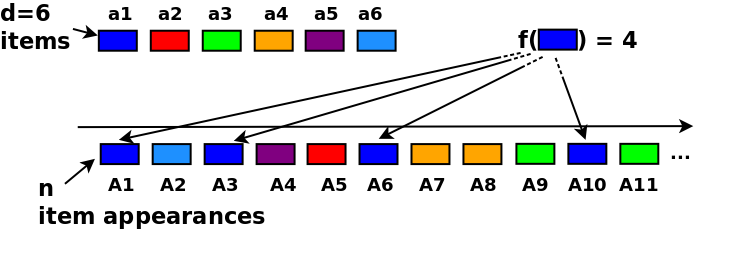
\includegraphics[scale=0.32]{plots/fi1}
 \label{fig:fi1}
\end{figure}

\framebreak

\begin{figure}
  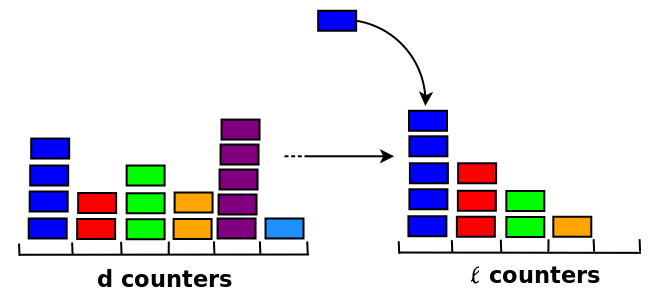
\includegraphics[scale=0.35]{plots/fi2}
 \label{fig:fi2}
\end{figure}

\framebreak

\begin{figure}
  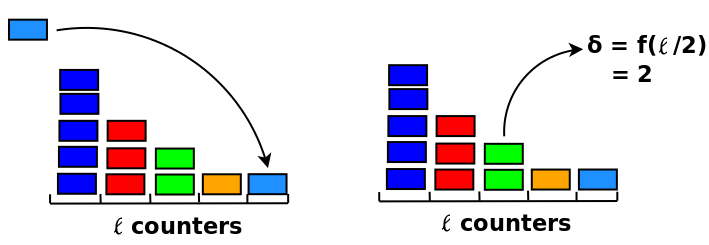
\includegraphics[scale=0.32]{plots/fi3}
 \label{fig:fi3}
\end{figure}

\framebreak

\begin{figure}
  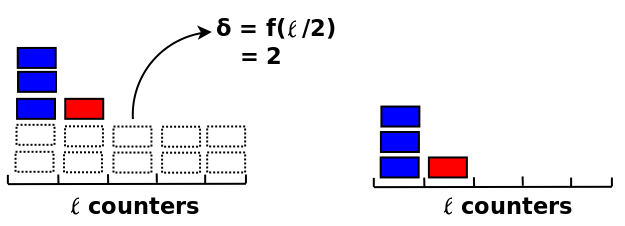
\includegraphics[scale=0.32]{plots/fi4}
 \label{fig:fi4}
\end{figure}

\framebreak

\begin{figure}
  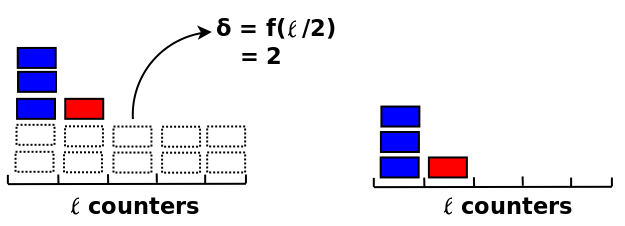
\includegraphics[scale=0.3]{plots/fi5}
 \label{fig:fi5}
\end{figure}

\framebreak

\begin{figure}
  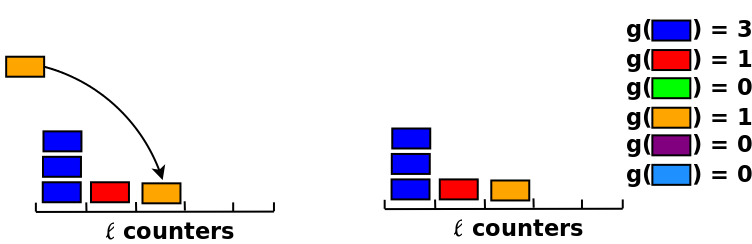
\includegraphics[scale=0.3]{plots/fi6}
 \label{fig:fi5}
\end{figure}

\textcolor{dgreen}{Claim.} 
For each item type $i$,
\begin{itemize}
	\item $g_{i}$ is a \textcolor{red}{good} approximation for its
  true frequency $f_{i}$ (even in the case of $g_{i}$ = 0),
	\item \textcolor{red}{'Good':} $|f_{i} - g_{i} | \leq n/\ell$.
\end{itemize}         

\framebreak

\begin{proof}
\begin{itemize}
	\item Each item-type is deleted \textcolor{dgreen}{at most} once per iteration:
		\begin{itemize}\item $g_{i} \leq f_{i}$\end{itemize}
	\item Each counter is decreased by at most $\delta_{t}$ at time $t$:
		\begin{itemize}\item $g_{i} \geq f_{i} - \sum_{t} \delta_{t} \Leftrightarrow f_{i} - g_{i} \leq \sum_{t} \delta_{t}$\end{itemize}
	\item Putting this together:
		\begin{itemize}
			\item $0 \leq \sum_{i}g_{i} \leq \sum_{t} 1 - (\ell/2)
				\cdot \delta_{t} = n - (\ell/2) \cdot \sum_{t} \delta_{t}$
			\item $\sum_{t} \delta_{t} \leq 2n/\ell$
		\end{itemize}
	\item Set $\ell = 2/\varepsilon$:
		\begin{itemize}\item $|f_{i} - g_{i}| \leq \varepsilon n$.\end{itemize}
\end{itemize}
\end{proof}

\framebreak

%\textbf{Proof (cont.):}

%\begin{itemize}
   %\item \textcolor{gray}{Each item-type is deleted at most once per iteration:}
   %\begin{itemize} \item \textcolor{gray}{$f_{i} - g_{i} \leq t$, where $t$ is the number of deleted items.}\end{itemize}
   %\item $\ell$ items are deleted in every batch, and the total number of
   %deleted items is \textcolor{red}{upper-bounded} by $n$, therefore:
   %\begin{itemize} \item $t\ell \leq n$, or $t \leq n/\ell$\cite{Misra82}.\end{itemize} 
\textcolor{gray}{\ldots What is the intuition of the following? \ldots}

\begin{itemize}
  \item If one sets $\ell > 1/\varepsilon$,
  \begin{itemize} \item Then any item that appears \textcolor{dgreen}{more than}
  $\varepsilon n$ times in the stream \textcolor{red}{must} appear in
  the final sketch.\end{itemize}
\end{itemize}
 
\end{frame}

%%%%%%%%%%%%%%%%%%%%%%%%%%%%%%%%%%%%%%%%%%%%%%%%%%%%%%%%%%%%%%%%%
% Frequent directions section
%%%%%%%%%%%%%%%%%%%%%%%%%%%%%%%%%%%%%%%%%%%%%%%%%%%%%%%%%%%%%%%%%

\begin{frame}{Content}
\begin{itemize}
\item \textcolor{gray}{Background}
\item \textcolor{gray}{Related work}
\item Frequent directions
\item \textcolor{gray}{Experiments and Results}
\item \textcolor{gray}{Conclusion}
\end{itemize}
\end{frame}

%%%%%%%%%%%%%%%%%%%%%%%%%%%%%%%%%%%%%%%%%%%%%%%%%%%%%%%%%%%%%%%%%%%%%%%%%%%%%%%%%%%%%%%%%%%%%

\begin{frame}[allowframebreaks=1]{The \textit{Frequent-directions} algorithm}

%\begin{itemize}
%  \item It allows for the process to be \textcolor{red}{inverted}
%  \begin{itemize}
%    \item Prescribe the threshold $t$ \textcolor{dgreen}{in advance} and find the space spanned by all
%vectors $x$, such that $\vectornorm{Ax} \geq t$.
%    \item In this setting, computing the SVD is \textcolor{red}{not necessary} anymore!
%   \end{itemize}
%\end{itemize}

%\framebreak
Represent the \textcolor{dgreen}{frequency} of a direction (unit vector):
\begin{itemize}
  \item Assume the directions of $A$ are \textcolor{red}{indicator vectors} of the items: \\
  \begin{center}
  \vspace{2 mm}
  $A = \begin{pmatrix}
       1 & 0 & 0 & 0\\[0.3em] 
       0 & 1 & 0 & 0\\[0.3em]
       0 & 0 & 1 & 0\\[0.3em]
       0 & 1 & 0 & 0
     \end{pmatrix}$
  \end{center}
  \item Frequency of second item $e_2 = (0,1,0,0)^T$:
  $ \vectornorm{Ae_2}^2 = \vectornorm{(0,1,0,1)^T} ^2= 0^2 + 1^2 + 0^2 + 1^2 = 2$. 
  \item Generalize the directions to unit vector $\{x : \vectornorm{x}=1\} $ and the \textcolor{dgreen}{frequency} of a direction is $\vectornorm{Ax}^2$.
\end{itemize}

\framebreak
Connection to SVD of $A$:
\begin{itemize}
  \item $A = U\Sigma V^T \Leftrightarrow U^TA = \Sigma V^T \Leftrightarrow Au = \sigma v$.
  \item $\vectornorm{Au}^2 = \vectornorm{\sigma v}^2 = \sigma^2$.
\end{itemize}
  \vspace{2 mm}
Change $u$ to $x$: \\
  \vspace{2 mm}

The \textcolor{dgreen}{frequency} of a direction is indicated by the square of corresponding singular value $\sigma^2$.

\framebreak
The algorithm:
  \begin{algorithmic}
    \State \textbf{Input}: $\ell$, $A \in \mathbb{R}^{n\times m}$
    \State $B \leftarrow $ all zeros matrix $\in \mathbb{R}^{\ell\times m}$
    \For{$i =1,\ldots,n$} 
    \State Insert $i^{th}$ row of $A$ into zero valued row of $B$
    \If {$B$ has no zero valued rows}
      \State $[U,\Sigma,V] \leftarrow SVD(B)$
      \textcolor{gray}{\State $C \leftarrow \Sigma V^T$ // for proof}
      \State $\delta \leftarrow \sigma_{\ell/2}^2$
      \State $\breve{\Sigma} \leftarrow \sqrt{\max(\Sigma^2-I_\ell\delta,0)}$
      \State $B\leftarrow \breve{\Sigma}V^T$
    \EndIf
    \EndFor
  \end{algorithmic}
  
\framebreak

\begin{figure}
  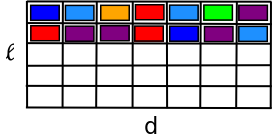
\includegraphics[scale=0.45]{plots/fd1}
 \label{fig:fd1}
\end{figure}

\framebreak

\begin{figure}
  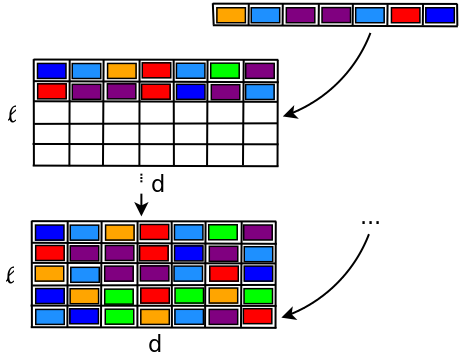
\includegraphics[scale=0.35]{plots/fd2}
 \label{fig:fd2}
\end{figure}

\framebreak

\begin{figure}
  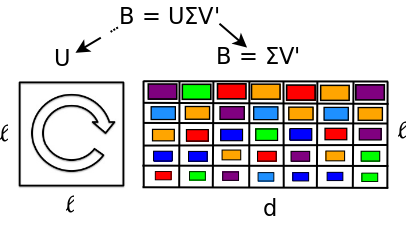
\includegraphics[scale=0.45]{plots/fd3}
 \label{fig:fd3}
\end{figure}

\framebreak

\begin{figure}
  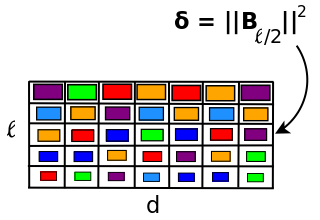
\includegraphics[scale=0.4]{plots/fd4}
 \label{fig:fd4}
\end{figure}

\framebreak

\begin{figure}
  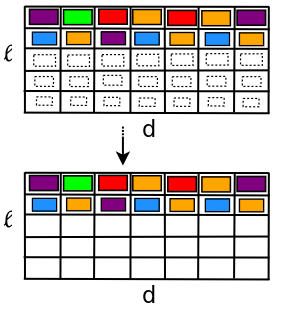
\includegraphics[scale=0.375]{plots/fd5}
 \label{fig:fd5}
\end{figure}  

\framebreak

\begin{figure}
  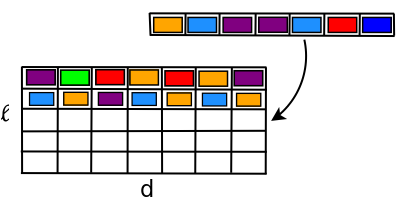
\includegraphics[scale=0.4]{plots/fd6}
 \label{fig:fd6}
\end{figure} 

\end{frame}


\begin{frame}[allowframebreaks=1]{Frequent direction example}

\begin{align}
  A = \begin{pmatrix}
       0.9387 & 0.3447 \\[0.3em] 
       0.7605 & 0.6493 \\[0.3em]
       0.5858 & 0.8104 \\[0.3em]
       0.3413 & 0.9400
     \end{pmatrix} 
  \rightarrow
  B = \begin{pmatrix}
      0  & 0  \\[0.3em] 
       0 & 0
     \end{pmatrix} \nonumber
\end{align}

\framebreak

\begin{align}
  A = \begin{pmatrix}
       0.9387 & 0.3447 \\[0.3em] 
       0.7605 & 0.6493 \\[0.3em]
       0.5858 & 0.8104 \\[0.3em]
       0.3413 & 0.9400
     \end{pmatrix} 
  \rightarrow
  B = \begin{pmatrix}
       0.9387 & 0.3447 \\[0.3em] 
       0 & 0
     \end{pmatrix} 
\end{align}

\framebreak

\begin{align}
  A = \begin{pmatrix}
       0.9387 & 0.3447 \\[0.3em] 
       0.7605 & 0.6493 \\[0.3em]
       0.5858 & 0.8104 \\[0.3em]
       0.3413 & 0.9400
     \end{pmatrix} 
  \rightarrow
  B = \begin{pmatrix}
       0.9387 & 0.3447 \\[0.3em] 
       0.7605 & 0.6493
     \end{pmatrix} 
\end{align}

\framebreak
 $[U,\Sigma,V] \leftarrow SVD(B)$
\begin{align}
  B = \begin{pmatrix}
       0.9387 & 0.3447 \\[0.3em] 
       0.7605 & 0.6493
     \end{pmatrix} = \hspace{7cm} \nonumber  \\
\nonumber  \\
     \begin{pmatrix}
        \bovermat{U}{-0.7071 & -0.7071} \\[0.3em] 
       -0.7071 & 0.7071
     \end{pmatrix} 
    \begin{pmatrix}
       \bovermat{$\Sigma$}{1.3920 & 0.0000}\\[0.3em] 
       0.0000 & 0.2495
     \end{pmatrix} 
    \begin{pmatrix}
       \bovermat{$V^T$}{-0.8632 & -0.5049} \\[0.3em] 
       -0.5049 & 0.8632
     \end{pmatrix}   \nonumber
\end{align}

$\delta \leftarrow \sigma_{\ell/2}^2$
\begin{align}
   \ell/2 = 1, \delta = 1.3920^2 \nonumber
\end{align}

\framebreak
$\breve{\Sigma} \leftarrow \sqrt{\max(\Sigma^2-I_\ell\delta,0)}$
\begin{align}
 \breve\Sigma=\sqrt{\max(
      \begin{pmatrix}
       \bovermat{$\Sigma^2$}{1.3920^2 & 0.0000}\\[0.3em] 
       0.0000 & 0.2495^2
     \end{pmatrix} - 
      \begin{pmatrix}
       \bovermat{$I\delta$}{1.3920^2 & 0.0000}\\[0.3em] 
       0.0000 & 1.3920^2
     \end{pmatrix},0)} 
   \nonumber
\end{align}
$B\leftarrow \breve{\Sigma}V^T$
\begin{align}
  B = 
    \begin{pmatrix}
       \bovermat{$\breve\Sigma$}{0.0000 & 0.0000}\\[0.3em] 
       0.0000 & 0.0000
     \end{pmatrix}   
    \begin{pmatrix}
       \bovermat{$V$}{-0.8632 & -0.5049} \\[0.3em] 
       -0.5049 & 0.8632
     \end{pmatrix} ^T 
 = \begin{pmatrix}
       0 & 0 \\[0.3em] 
       0 & 0
      \end{pmatrix}  \nonumber 
\end{align}

\framebreak
\begin{align}
  A = \begin{pmatrix}
       0.9387 & 0.3447 \\[0.3em] 
       0.7605 & 0.6493 \\[0.3em]
       0.5858 & 0.8104 \\[0.3em]
       0.3413 & 0.9400
     \end{pmatrix} 
  \rightarrow
  B = \begin{pmatrix}
       0.5858 & 0.8104 \\[0.3em]
       0 & 0
     \end{pmatrix} 
\end{align}


\framebreak
\begin{align}
  A = \begin{pmatrix}
       0.9387 & 0.3447 \\[0.3em] 
       0.7605 & 0.6493 \\[0.3em]
       0.5858 & 0.8104 \\[0.3em]
       0.3413 & 0.9400
     \end{pmatrix} 
  \rightarrow
  B = \begin{pmatrix}
       0.5858 & 0.8104 \\[0.3em]
       0.3413 & 0.9400
     \end{pmatrix} 
\end{align}
\end{frame}


\begin{frame}[allowframebreaks=1]{Properties of the sketch matrix $B$}
In summary:
\begin{itemize}
  \item $A^TA \succeq B^TB \succeq 0$.
  \vspace{2 mm}
  \item $ ||A^TA - B^TB || \leq 2|| A||_f^2/\ell$. 
  \vspace{2 mm}
  \item Let $A = [A_1;A_2]$ and $B_1$, $B_2$ is the sketches of $A_1$ and $A_2$. A sketch $C$ of $B=[B_1;B_2]$ can be shown that:\\
  {\color{blue}\begin{align}
    ||A^TA - C^TC || \leq 2|| A||_f^2/\ell. \nonumber 
  \end{align}}
\end{itemize}
\end{frame}
%  \vspace{2 mm}
%1. $A^TA \succeq B^TB \succeq 0$. 
%\footnotesize
%\begin{proof}
%  {\color{blue}\begin{flalign}
%   & B^TB \succeq 0 \Leftrightarrow x^TB^TBx \geq 0 \Leftrightarrow \vectornorm{Bx}^2 \geq 0. && \nonumber \\
%   & A^TA \succeq B^TB  \Leftrightarrow x^T(A^TA-B^TB)x \geq 0 \Leftrightarrow \vectornorm{Ax}^2 -\vectornorm{Bx}^2 \geq 0. \nonumber &&
%  \end{flalign}}
%  {\color{blue}\begin{flalign}
%    \vectornorm{Ax}^2 -\vectornorm{Bx}^2 &= \sum_{i=1}^n[\langle A_i, x \rangle^2 + ||B^{i-1}x||^2 - ||B^{i}x||^2] \nonumber &&\\
%    &= \sum_{i=1}^n[||C^ix||^2 - ||B^{i}x||^2]= \sum_{i=1}^n[x^T(C^{i^T}C^i-B^{i^T}B^i)x] \nonumber &&\\
%    &= \sum_{i=1}^n[x^T(V\Sigma^T\Sigma V^T-V\breve{\Sigma}^T\breve{\Sigma} V^T)x] 
%    = \sum_{i=1}^n[x^TV(\Sigma^2 -\breve{\Sigma}^2)V^Tx] \geq 0. && \nonumber
%  \end{flalign}}
%\end{proof}


%\framebreak

%\normalsize
%  \vspace{2 mm}
%2. $ ||A^TA - B^TB || \leq 2|| A||_f^2/\ell$. 
%\footnotesize
%\begin{proof}
%  {\color{blue}\begin{flalign}
%    &||A^TA - B^TB || \leq \sum_{i=1}^n\delta_i \leq 2||A||_f^2/\ell. && \nonumber  
%  \end{flalign}}
%  {\color{blue}\begin{flalign}
%    ||A^TA - B^TB || &= \sigma_{max}(A^TA - B^TB) = x^T(A^TA-B^TB)x = \vectornorm{Ax}^2 -\vectornorm{Bx}^2  \nonumber && \\
%    &= \sum_{i=1}^n[||C^ix||^2 - ||B^{i}x||^2] \leq \sum_{i=1}^n[||C^{i^T}C^i - B^{i^T}B^i||] && \nonumber \\
%    &= \sum_{i=1}^n[||V(\Sigma^2 -\breve{\Sigma}^2) V^T||] =  \sum_{i=1}^n \delta_i. %\nonumber && 
%  \end{flalign}}
%\end{proof}

%\framebreak

%\normalsize
%  \vspace{2 mm}
%2. $ ||A^TA - B^TB || \leq 2|| A||_f^2/\ell$. 
%\footnotesize
%\begin{proof}
%  \begin{flalign}
%    &||A^TA - B^TB || \leq \sum_{i=1}^n\delta_i \leq 2||A||_f^2/\ell. && \nonumber 
%  \end{flalign}
%  {\color{blue}\begin{flalign}
%    ||B^n||_f^2 &= \sum_{i=1}^n[||B^{i-1}x||_f^2 - ||B^{i}||_f^2] = \sum_{i=1}^n[(||C^i||_f^2 - ||B^{i-1}x||_f^2) - (||C^i||_f^2 - ||B^{i}||_f^2)]. && \nonumber \\
%     &= \sum_{i=1}^n ||A_i||_f^2 - tr(C^{i^T}C^i - B^{i^T}B^i) = ||A||_f^2 - \sum_{i=1}^ntr(V(\Sigma^{i^2} -\breve{\Sigma}^{i^2}) V^T) && \nonumber \\
%     &= ||A||_f^2 - \sum_{i=1}^ntr(\Sigma^{i^2} -\breve{\Sigma}^{i^2}) \leq ||A||_f^2 - (\ell/2)\sum_{i=1}^n\delta_i \nonumber.
%  \end{flalign}}
%  {\color{blue}\begin{flalign}
%    \sum_{i=1}^n\delta_i \leq 2(||A||_f^2 - ||B||_f^2)/\ell \leq 2||A||_f^2/\ell. && \nonumber
%  \end{flalign}}
%\end{proof}
%\normalsize


%\framebreak


%%%%%%%%%%%%%%%%%%%%%%%%%%%%%%%%%%%%%%%%%%%%%%%%%%%%%%%%%%%%%%%%%
% Experiment section
%%%%%%%%%%%%%%%%%%%%%%%%%%%%%%%%%%%%%%%%%%%%%%%%%%%%%%%%%%%%%%%%%

\begin{frame}{Content}
\begin{itemize}
\item \textcolor{gray}{Background}
\item \textcolor{gray}{Related work}
\item \textcolor{gray}{Frequent directions}
\item Experiments and Results
\item \textcolor{gray}{Conclusion}
\end{itemize}
\end{frame}


\begin{frame}[allowframebreaks=1]{Experiments}
Synthetic data $A \in \mathbb{R}^{n\times m}$
\begin{itemize}
  \item $A = SDU + N/\zeta$.
  \item $S \in \mathbb{R}^{n\times d},\quad S_{i,j} \sim \mathcal{N}(0,1)$.
  \item $D \in \mathbb{R}^{d\times d},\quad D_{i,i} = 1 - (i-1)/d$.
  \item $U \in \mathbb{R}^{d\times m}, \quad UU^T=I_d$.
  \item $c_1 \leq \zeta \leq c_2, \quad c_1 \approx 1,c_2 \approx 1$.
\end{itemize}
$A$ contains $d$ dimensional signal and $m$ dimensional noise, and is recoverable by spectral methods \cite{Vershynin11}.


\framebreak
Error against sketch size with $n=10000, m=1000, d=50$.
\begin{figure}
  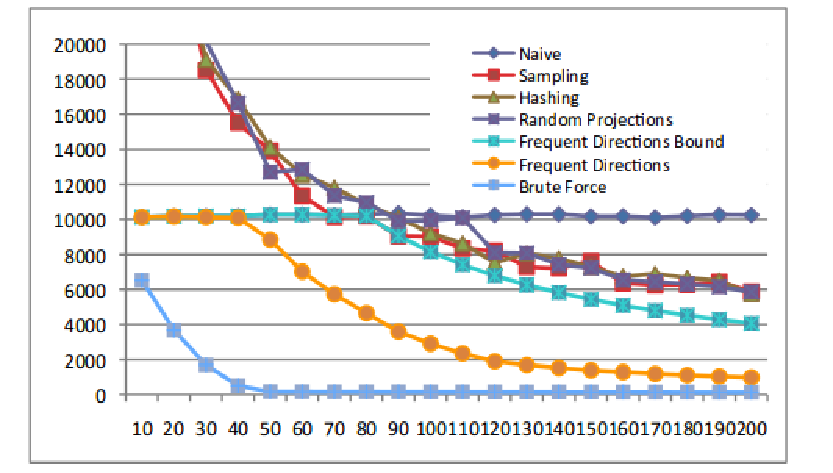
\includegraphics[scale=0.6]{plots/acc}
 \label{fig:fp}
\end{figure}

\framebreak
Running time. \\
Left figure shows comparison with other techniques and right figure shows the linear behavior in $n$ and $m$.
\begin{figure}
  \subfigure{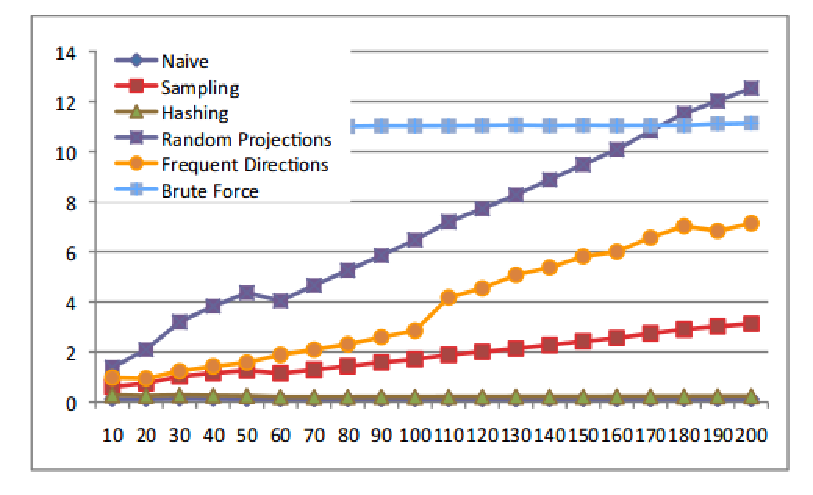
\includegraphics[scale=0.35]{plots/time1}}
  \subfigure{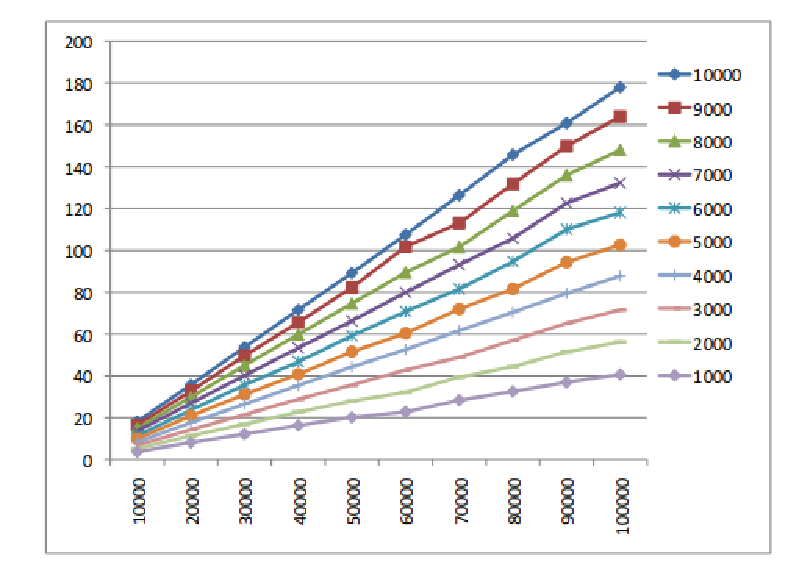
\includegraphics[scale=0.35]{plots/time2}}
 \label{fig:fgtree}
\end{figure}
\end{frame}

\begin{frame}[allowframebreaks=1]{More experiments}
\begin{figure}
  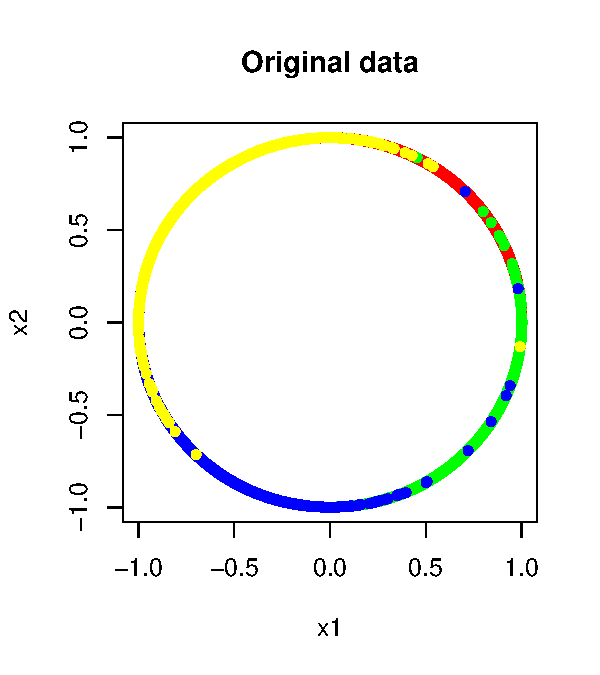
\includegraphics[scale=0.6]{plots/data_and_sketch}
 \label{fig:fp}
\end{figure}

\framebreak

{\color{blue}\begin{flalign}
  A^TA = \times\begin{pmatrix}
       4979.0 & 75.7 \\[0.3em] 
       75.7 & 5021.0
     \end{pmatrix} 
  B^TB = \begin{pmatrix}
       4979.0 & 75.6 \\[0.3em] 
       75.6 & 5020.9
     \end{pmatrix} \nonumber  
\end{flalign}}

{\color{blue}\begin{flalign}
  B = \begin{pmatrix}
       43.0030 & 56.8110 \\[0.3em] 
       -55.9340 & 32.3390 \\[0.3em] 
       0.5011 & 0.8654 \\[0.3em] 
       -0.9427 & -0.3336 \\[0.3em] 
         0 & 0 \\[0.3em] 
	 \vdots & \vdots 
     \end{pmatrix} \nonumber
\end{flalign}}
\end{frame}

\begin{frame}{Conclusion}
\begin{itemize}
  \item In terms of $|| A^TA - B^TB||$, the proposed sketching algorithm is \textcolor{red}{more accurate} than sampling, hashing and random projections.
  \item The proposed algorithm runs reasonably fast
  \begin{itemize}\item in fact, \textcolor{red}{faster} than random projection, slower than sampling.\end{itemize}
  \item The proposed algorithm is \textcolor{red}{linear} in the scale of the input size.
\end{itemize}
\end{frame}

\begin{frame}{Thank you!}
\begin{itemize}
  \item \LARGE{Questions?}
\end{itemize}
\end{frame}


%%%%%%%%%%%%%%%%%%%%%%%%%%%%%%%%%%%%%%%%%%%%%%%%%%%%%%%%%%%%%%%%%%%%%%%%%%%%%%%%%%%%%%

\bibliographystyle{plain}
\begin{frame}[allowframebreaks=1]{References}
\small
\bibliography{presentation}
\end{frame}

\end{document}
